\section{Описание}
Нужно разработать поискового робота, способного обходить веб-страницы и сохранять их содержимое в базу данных. В качестве базы данных была выбрана, упомянутая в условии лабораторной работы, \textbf{MongoDB} -- документоориентированная NoSQL-система, которая подходит для хранения html-страниц.

Было принято решение использовать \textbf{sitemap} выбранных ресурсов для сбора URL. Sitemap -- это XML-файл, который предоставляют сайты поисковикам для показа страниц, доступных для индексации. Sitemap содержит готовый список всех страниц сайта -- не нужно рекурсивно обходить сайты. В sitemap указывается дата последнего изменения страницы (lastmod) - можно легко отслеживать изменения. Также URL уже нормализованы.

Необходимо удовлетворить условию и сделать так, чтобы робот мог останавливаться и продолжать работу, а также переобкачивать страницы. Также нужен конфигурационный yaml-файл.

\pagebreak

\section{Исходный код}

Робот написан на Python с использованием: \texttt{requests} для HTTP-запросов, \texttt{PyYAML} для чтения конфигурации, \texttt{pymongo} для работы с MongoDB, \texttt{xml.etree.ElementTree} для парсинга XML-файлов sitemap.

\vspace{1 em}
\noindent\textbf{yaml файл.} При работе с sitemap источника stopgame.ru была замечена особенность: указанные в нем URL не соответствовали фактическим: \\
 указано \texttt{https://stopgame.ru/news/64976/}, а реальные были вида \\
 \texttt{https://stopgame.ru/newsdata/64976/}. Для этого в конфигурационный файл была добавлена логика \texttt{url\_transforms}, позволяющая при помощи регулярных выражений приводить ссылки одного вида к другому, чтобы решить эту проблему. Поля конфигурационного файла robot.yml:

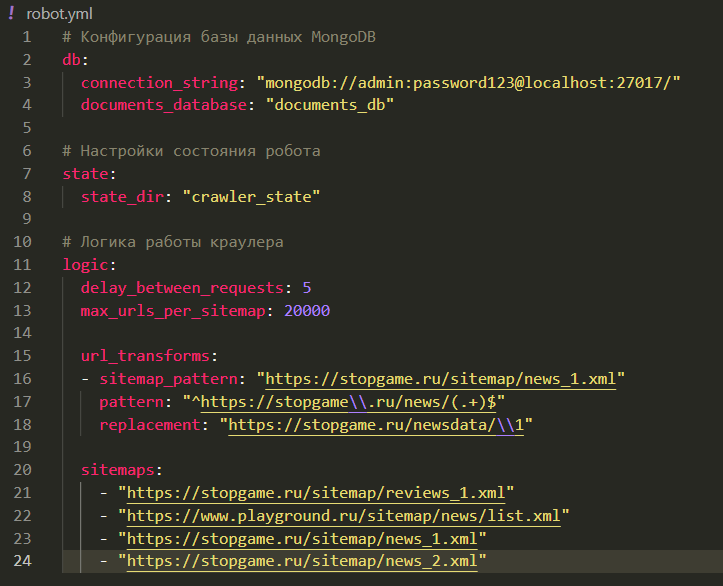
\includegraphics[width=\textwidth, height=\textheight, keepaspectratio]{pics/config.png}

\begin{itemize}
    \item \texttt{db} -- настройки БД:
    \begin{itemize}
        \item \texttt{connection\_string} -- строка подключения к MongoDB
        \item \texttt{documents\_database} -- название БД
    \end{itemize}
    
    \item \texttt{state} -- управление состоянием:
    \begin{itemize}
        \item \texttt{state\_dir} -- директория для хранения файлов состояния
    \end{itemize}
    
    \item \texttt{logic} -- секция логики работы:
    \begin{itemize}
        \item \texttt{delay\_between\_requests} -- задержка между загрузками страниц в секундах
        \item \texttt{max\_urls\_per\_sitemap} -- максимальное количество URL, обрабатываемых из одного sitemap (0 — если не нужны ограничения)
        \item \texttt{interval\_seconds} -- интервал переобкачки
        \item \texttt{sitemaps} -- список URL sitemap-файлов для обработки
        \item \texttt{url\_transforms} -- список правил трансформации URL
    \end{itemize}
\end{itemize}

\vspace{1 em}
\noindent\textbf{Сохранения состояния.} Состояние робота хранится в вспомогательных json-файлах:

\begin{itemize}
    \item \texttt{queue.json} -- текущая очередь URL на обкачку/переобкачку. При остановке робота очередь сохраняется. Так что робот продолжит работу с того места, где остановился.
    
    \item \texttt{sitemap\_cache.json} -- кэш данных из sitemap. Это словарь, ключ — URL страницы, значение -- дата последнего изменения (\texttt{lastmod}) из sitemap. Он нужен чтобы при возобновлении работы заново не парсить все URL из sitemap. Обновляется периодически.
\end{itemize}


Оба файла сохраняются в \texttt{state\_dir}. При нажатии (Ctrl+C) робот сохраняет состояние и завершает работу.


\vspace{1 em}
\noindent\textbf{Алгоритм работы робота.} Робот находится в бесконечном цикле:

Если очередь пуста (первый запуск или все URL обработаны):
\begin{enumerate}
    \item Для каждого sitemap из конфигурации:
    \begin{itemize}
        \item Загружается и парсится XML-файл
        \item Извлекаются URL и даты последнего изменения (\texttt{lastmod})
        \item Применяются правила трансформации (если заданы)
        \item Данные сохраняются в \texttt{sitemap\_cache.json}
    \end{itemize}
\end{enumerate}

Для каждого URL из кэша sitemap:
\begin{enumerate}
    \item Если URL отсутствует в БД -- добавляется в очередь
    \item Для уже обкаченных URL -- проверяются два условия:
    \begin{itemize}
        \item Прошло ли достаточно времени с последней обкачки (сравнение с \texttt{interval\_seconds})
        \item Изменилась ли страница (сравнение \texttt{lastmod} из sitemap с временем последней обкачки из БД)
        \item Если оба условия верны - нужно переобкачать
    \end{itemize}
\end{enumerate}

Обработка очереди:
\begin{enumerate}
    \item URL извлекаются из очереди по одному
    \item Для каждого URL:
    \begin{itemize}
        \item Загружается html-файл
        \item Извлекается название источника (домен из URL)
        \item Формируется документ БД с полями:
        \begin{itemize}
            \item \texttt{\_id} — уникальный числовой идентификатор
            \item \texttt{url} — нормализованный URL (после трансформации)
            \item \texttt{html} — сырой html-код
            \item \texttt{source\_name} — название источника
            \item \texttt{crawl\_time} — время обкачки в формате Unix timestamp
        \end{itemize}
        \item Документ сохраняется в БД
    \end{itemize}
    \item Выжидаем паузу \texttt{delay\_between\_requests}
\end{enumerate}

Когда очередь пустеет робот возвращается к обновлению кэша sitemap, начиная новый цикл. Если изменений в sitemap нет -- робот переходит в режим ожидания до появления новых данных или изменения существующих.

Для выбранных источников в файлах \texttt{robots.txt} не было обнаружено вежливого интервала для обкачки, так что она осуществлялась с интервалом в 5 секунд (приходилось оставлять робота работать по ночам)

\pagebreak

